% Contenidos del capítulo.
% Las secciones presentadas son orientativas y no representan
% necesariamente la organización que debe tener este capítulo.

\section{Diagramas de análisis}

\subsection{Diagrama de casos de uso}

Para representar las interacciones entre los diferentes actores del sistema se ha elaborado el diagrama de casos de uso mostrado en la Figura~\ref{fig:casos_uso}. 
Este permite visualizar de forma general las funcionalidades principales y la relación entre el cliente, el administrador y el \textit{bot de Telegram}.

\begin{figure}[H]
    \centering
    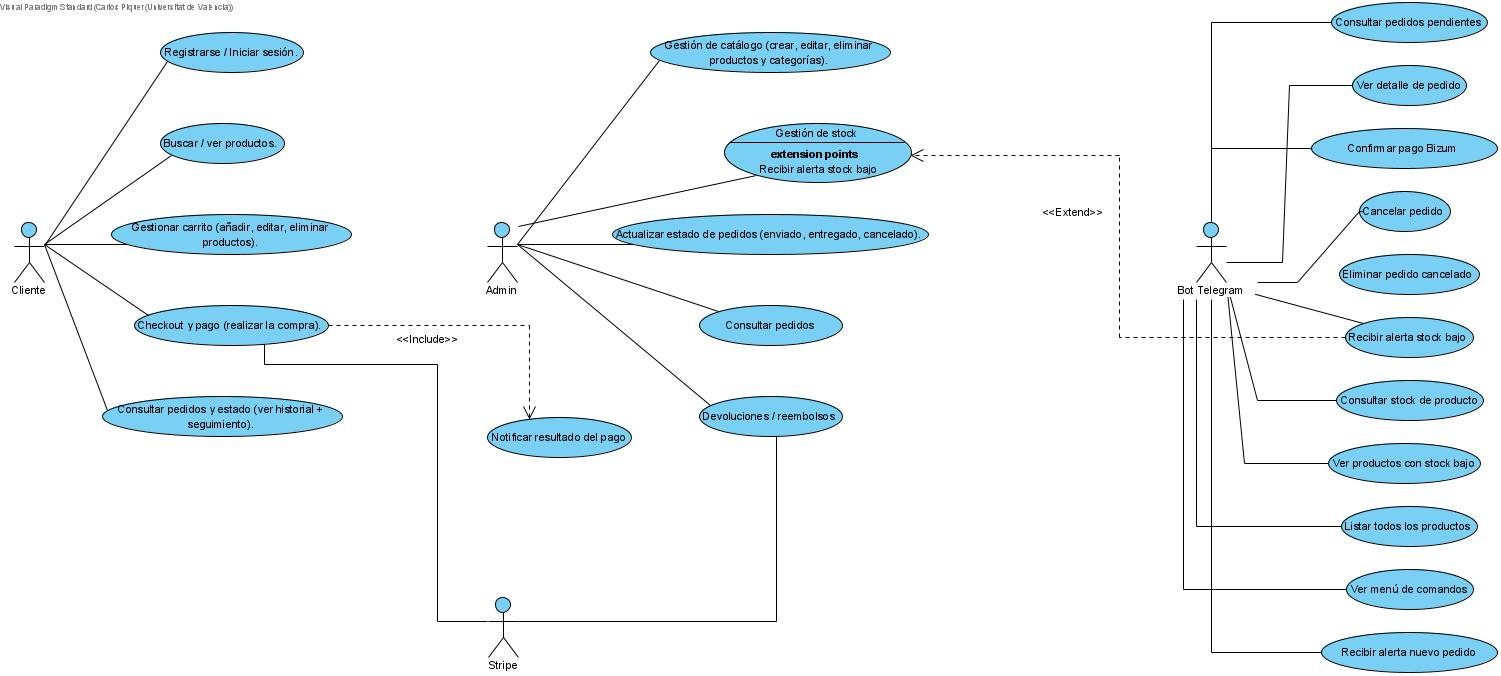
\includegraphics[height=1\textwidth, width=1.05\textwidth, keepaspectratio]{figs/casos_de_uso_goodv2.jpg}
    \caption{Diagrama de casos de uso del sistema.}
    \label{fig:casos_uso}
\end{figure}
\clearpage

\subsection{Especificación de casos de uso}

A continuación se especifica, en formato tabular, el detalle de cada uno de los casos de uso identificados en el diagrama anterior. Los casos de uso se agrupan por actor: cliente, administrador, Stripe y bot de Telegram.

\subsubsection{CU-01 Registrarse / iniciar sesión}

\begin{table}[H]
\centering
\small
\begin{tabular}{|m{0.28\textwidth}|m{0.65\textwidth}|}
\hline
\textbf{Nombre} & CU-01 Registrarse / iniciar sesión \\ \hline
\textbf{Actor(es)} & Cliente \\ \hline
\textbf{Descripción} & El cliente puede registrarse como nuevo usuario o iniciar sesión con sus credenciales. \\ \hline
\textbf{Precondiciones} & El sistema debe estar accesible. Para iniciar sesión, el usuario debe estar registrado previamente. \\ \hline
\textbf{Postcondiciones} & El cliente queda autenticado y accede a las funcionalidades reservadas para usuarios registrados. \\ \hline
\textbf{Flujo principal} & 1. El cliente accede a la pantalla de registro o inicio de sesión. \newline 2. Introduce sus datos (correo electrónico y contraseña). \newline 3. El sistema valida las credenciales. \newline 4. El cliente queda autenticado y es redirigido al inicio. \\ \hline
\textbf{Flujos alternativos} & 3.a Credenciales incorrectas $\rightarrow$ el sistema muestra un mensaje de error. \newline 3.b Correo ya registrado (en registro) $\rightarrow$ el sistema informa del duplicado. \\ \hline
\textbf{Requisitos funcionales relacionados} & RF-01 \\ \hline
\end{tabular}
\caption{Especificación del caso de uso CU-01 — Registrarse / iniciar sesión.}
\end{table}

\subsubsection{CU-02 Buscar / ver productos}

\begin{table}[H]
\centering
\small
\begin{tabular}{|m{0.28\textwidth}|m{0.65\textwidth}|}
\hline
\textbf{Nombre} & CU-02 Buscar / ver productos \\ \hline
\textbf{Actor(es)} & Cliente \\ \hline
\textbf{Descripción} & El cliente explora el catálogo, aplica filtros por categoría y precio, y realiza búsquedas por nombre de producto. \\ \hline
\textbf{Precondiciones} & El catálogo debe contener productos disponibles. \\ \hline
\textbf{Postcondiciones} & El cliente visualiza los productos que cumplen los criterios de búsqueda o filtrado. \\ \hline
\textbf{Flujo principal} & 1. El cliente accede a la sección de catálogo. \newline 2. Aplica filtros opcionales o introduce un término de búsqueda. \newline 3. El sistema devuelve y muestra los resultados correspondientes. \\ \hline
\textbf{Flujos alternativos} & 3.a Ningún producto coincide con los criterios $\rightarrow$ el sistema muestra un mensaje informativo. \\ \hline
\textbf{Requisitos funcionales relacionados} & RF-02 \\ \hline
\end{tabular}
\caption{Especificación del caso de uso CU-02 — Buscar / ver productos.}
\end{table}

\subsubsection{CU-03 Gestionar carrito}

\begin{table}[H]
\centering
\small
\begin{tabular}{|m{0.28\textwidth}|m{0.65\textwidth}|}
\hline
\textbf{Nombre} & CU-03 Gestionar carrito \\ \hline
\textbf{Actor(es)} & Cliente \\ \hline
\textbf{Descripción} & El cliente añade productos al carrito, modifica cantidades o elimina artículos. \\ \hline
\textbf{Precondiciones} & El cliente debe estar autenticado y el catálogo debe estar operativo. \\ \hline
\textbf{Postcondiciones} & El carrito queda actualizado con los productos y cantidades seleccionados. \\ \hline
\textbf{Flujo principal} & 1. El cliente selecciona un producto del catálogo. \newline 2. Lo añade al carrito. \newline 3. La WebApp actualiza las unidades y el total del carrito. \newline 4. El cliente puede modificar cantidades o eliminar artículos. \newline 5. El sistema mantiene los datos sincronizados. \\ \hline
\textbf{Flujos alternativos} & 2.a Stock insuficiente $\rightarrow$ el sistema muestra un aviso. \newline 1.a El cliente no dispone de carrito activo $\rightarrow$ el sistema crea uno automáticamente. \\ \hline
\textbf{Requisitos funcionales relacionados} & RF-03 \\ \hline
\end{tabular}
\caption{Especificación del caso de uso CU-03 — Gestionar carrito.}
\end{table}

\clearpage

\subsubsection{CU-04 Checkout y pago}

\begin{table}[H]
\centering
\small
\begin{tabular}{|m{0.28\textwidth}|m{0.65\textwidth}|}
\hline
\textbf{Nombre} & CU-04 Checkout y pago \\ \hline
\textbf{Actor(es)} & Cliente, Stripe \\ \hline
\textbf{Descripción} & El cliente completa el proceso de compra introduciendo sus datos personales y de pago. El pago es procesado por la pasarela Stripe. Incluye CU-11 (\textit{Notificar resultado del pago}). \\ \hline
\textbf{Precondiciones} & El cliente debe estar autenticado y disponer de un carrito con productos. \\ \hline
\textbf{Postcondiciones} & El pedido queda registrado como pagado y se genera la factura correspondiente. \\ \hline
\textbf{Flujo principal} & 1. El cliente accede al checkout. \newline 2. Introduce sus datos personales y dirección de envío. \newline 3. Selecciona el método de pago. \newline 4. La WebApp crea el pedido en estado ``pendiente''. \newline 5. Stripe procesa el pago. \newline 6. Stripe notifica el resultado (CU-11). \newline 7. La WebApp confirma el pedido y genera la factura. \\ \hline
\textbf{Flujos alternativos} & 5.a Stripe requiere autenticación adicional (3D Secure). \newline 5.b Pago rechazado $\rightarrow$ el sistema muestra un mensaje de error y el pedido no se completa. \\ \hline
\textbf{Requisitos funcionales relacionados} & RF-04, RF-06 \\ \hline
\end{tabular}
\caption{Especificación del caso de uso CU-04 — Checkout y pago.}
\end{table}

\subsubsection{CU-05 Consultar pedidos y estado}

\begin{table}[H]
\centering
\small
\begin{tabular}{|m{0.28\textwidth}|m{0.65\textwidth}|}
\hline
\textbf{Nombre} & CU-05 Consultar pedidos y estado \\ \hline
\textbf{Actor(es)} & Cliente \\ \hline
\textbf{Descripción} & El cliente consulta el historial de sus pedidos anteriores y el estado actualizado de cada uno. \\ \hline
\textbf{Precondiciones} & El cliente debe estar autenticado y haber realizado al menos un pedido. \\ \hline
\textbf{Postcondiciones} & El cliente visualiza el historial de pedidos con sus estados actualizados. \\ \hline
\textbf{Flujo principal} & 1. El cliente accede a su área personal. \newline 2. Selecciona la sección de historial de pedidos. \newline 3. El sistema muestra el listado de pedidos con su estado y detalle. \\ \hline
\textbf{Flujos alternativos} & 3.a No existen pedidos $\rightarrow$ el sistema muestra un mensaje informativo. \\ \hline
\textbf{Requisitos funcionales relacionados} & RF-08 \\ \hline
\end{tabular}
\caption{Especificación del caso de uso CU-05 — Consultar pedidos y estado.}
\end{table}

\clearpage

\subsubsection{CU-06 Gestión de catálogo}

\begin{table}[H]
\centering
\small
\begin{tabular}{|m{0.28\textwidth}|m{0.65\textwidth}|}
\hline
\textbf{Nombre} & CU-06 Gestión de catálogo \\ \hline
\textbf{Actor(es)} & Administrador \\ \hline
\textbf{Descripción} & El administrador crea, edita y elimina productos y categorías del catálogo de la tienda. \\ \hline
\textbf{Precondiciones} & El administrador debe estar autenticado con permisos de administración. \\ \hline
\textbf{Postcondiciones} & Los cambios en el catálogo quedan reflejados de forma inmediata en la tienda. \\ \hline
\textbf{Flujo principal} & 1. El administrador accede al panel de administración. \newline 2. Selecciona la sección de catálogo. \newline 3. Crea, edita o elimina un producto o categoría. \newline 4. El sistema actualiza el catálogo. \\ \hline
\textbf{Flujos alternativos} & 3.a Datos del producto incompletos $\rightarrow$ el sistema solicita corrección. \newline 3.b Eliminación de producto con pedidos activos $\rightarrow$ el sistema muestra un aviso. \\ \hline
\textbf{Requisitos funcionales relacionados} & RF-05 \\ \hline
\end{tabular}
\caption{Especificación del caso de uso CU-06 — Gestión de catálogo.}
\end{table}

\subsubsection{CU-07 Gestión de stock}

\begin{table}[H]
\centering
\small
\begin{tabular}{|m{0.28\textwidth}|m{0.65\textwidth}|}
\hline
\textbf{Nombre} & CU-07 Gestión de stock \\ \hline
\textbf{Actor(es)} & Administrador \\ \hline
\textbf{Descripción} & El administrador actualiza manualmente el stock de los productos. Si el valor resultante es inferior al umbral configurado, se extiende el caso de uso con el envío automático de una alerta (CU-18). \\ \hline
\textbf{Precondiciones} & El administrador debe estar autenticado. \\ \hline
\textbf{Postcondiciones} & El stock del producto queda actualizado. Si el nuevo valor está por debajo del umbral, se genera una alerta automática. \\ \hline
\textbf{Flujo principal} & 1. El administrador accede al panel de administración. \newline 2. Selecciona un producto y modifica su valor de stock. \newline 3. El sistema guarda el nuevo valor. \\ \hline
\textbf{Flujos alternativos} & 3.a El nuevo stock es inferior al umbral $\rightarrow$ el sistema extiende con CU-18 (alerta de bajo stock). \\ \hline
\textbf{Requisitos funcionales relacionados} & RF-05, RF-07 \\ \hline
\end{tabular}
\caption{Especificación del caso de uso CU-07 — Gestión de stock.}
\end{table}

\subsubsection{CU-08 Actualizar estado de pedidos}

\begin{table}[H]
\centering
\small
\begin{tabular}{|m{0.28\textwidth}|m{0.65\textwidth}|}
\hline
\textbf{Nombre} & CU-08 Actualizar estado de pedidos \\ \hline
\textbf{Actor(es)} & Administrador \\ \hline
\textbf{Descripción} & El administrador actualiza el estado de los pedidos recibidos: enviado, entregado o cancelado. \\ \hline
\textbf{Precondiciones} & El administrador debe estar autenticado y deben existir pedidos en el sistema. \\ \hline
\textbf{Postcondiciones} & El estado del pedido queda actualizado en el sistema. \\ \hline
\textbf{Flujo principal} & 1. El administrador accede a la sección de pedidos. \newline 2. Selecciona un pedido concreto. \newline 3. Cambia el estado al valor correspondiente. \newline 4. El sistema guarda el nuevo estado. \\ \hline
\textbf{Flujos alternativos} & — No aplica. \\ \hline
\textbf{Requisitos funcionales relacionados} & RF-08 \\ \hline
\end{tabular}
\caption{Especificación del caso de uso CU-08 — Actualizar estado de pedidos.}
\end{table}

\clearpage

\subsubsection{CU-09 Consultar pedidos}

\begin{table}[H]
\centering
\small
\begin{tabular}{|m{0.28\textwidth}|m{0.65\textwidth}|}
\hline
\textbf{Nombre} & CU-09 Consultar pedidos \\ \hline
\textbf{Actor(es)} & Administrador \\ \hline
\textbf{Descripción} & El administrador consulta el listado completo de pedidos del sistema, con la posibilidad de filtrar por estado. \\ \hline
\textbf{Precondiciones} & El administrador debe estar autenticado. \\ \hline
\textbf{Postcondiciones} & El administrador visualiza el listado de pedidos con la información relevante. \\ \hline
\textbf{Flujo principal} & 1. El administrador accede a la sección de pedidos. \newline 2. Aplica filtros opcionales por estado. \newline 3. El sistema muestra el listado de pedidos. \\ \hline
\textbf{Flujos alternativos} & 3.a No hay pedidos $\rightarrow$ el sistema muestra un mensaje informativo. \\ \hline
\textbf{Requisitos funcionales relacionados} & RF-08 \\ \hline
\end{tabular}
\caption{Especificación del caso de uso CU-09 — Consultar pedidos.}
\end{table}

\subsubsection{CU-10 Devoluciones / reembolsos}

\begin{table}[H]
\centering
\small
\begin{tabular}{|m{0.28\textwidth}|m{0.65\textwidth}|}
\hline
\textbf{Nombre} & CU-10 Devoluciones / reembolsos \\ \hline
\textbf{Actor(es)} & Administrador \\ \hline
\textbf{Descripción} & El administrador gestiona las solicitudes de devolución o reembolso de pedidos. \\ \hline
\textbf{Precondiciones} & El administrador debe estar autenticado y debe existir un pedido susceptible de devolución. \\ \hline
\textbf{Postcondiciones} & El pedido queda marcado como devuelto o reembolsado y el stock se repone si procede. \\ \hline
\textbf{Flujo principal} & 1. El administrador accede al detalle de un pedido. \newline 2. Selecciona la opción de devolución o reembolso. \newline 3. El sistema actualiza el estado del pedido. \newline 4. Si procede, el stock de los artículos devueltos se restaura. \\ \hline
\textbf{Flujos alternativos} & 3.a El pedido no es elegible para devolución $\rightarrow$ el sistema muestra un aviso. \\ \hline
\textbf{Requisitos funcionales relacionados} & RF-08 \\ \hline
\end{tabular}
\caption{Especificación del caso de uso CU-10 — Devoluciones / reembolsos.}
\end{table}

\subsubsection{CU-11 Notificar resultado del pago}

\begin{table}[H]
\centering
\small
\begin{tabular}{|m{0.28\textwidth}|m{0.65\textwidth}|}
\hline
\textbf{Nombre} & CU-11 Notificar resultado del pago \\ \hline
\textbf{Actor(es)} & Stripe \\ \hline
\textbf{Descripción} & Stripe notifica a la WebApp el resultado del procesamiento del pago (confirmación o rechazo). Este caso de uso es incluido por CU-04 (\textit{Checkout y pago}). \\ \hline
\textbf{Precondiciones} & El cliente debe haber iniciado el proceso de pago en el checkout. \\ \hline
\textbf{Postcondiciones} & La WebApp recibe y procesa el resultado, actualizando el estado del pedido. \\ \hline
\textbf{Flujo principal} & 1. Stripe procesa la transacción. \newline 2. Stripe envía la notificación del resultado a la WebApp. \newline 3. La WebApp actualiza el estado del pedido en consecuencia. \\ \hline
\textbf{Flujos alternativos} & 2.a Error de comunicación $\rightarrow$ la WebApp reintenta la confirmación. \\ \hline
\textbf{Requisitos funcionales relacionados} & RF-04 \\ \hline
\end{tabular}
\caption{Especificación del caso de uso CU-11 — Notificar resultado del pago.}
\end{table}

\clearpage

\subsubsection{CU-12 Recibir alerta nuevo pedido}

\begin{table}[H]
\centering
\small
\begin{tabular}{|m{0.28\textwidth}|m{0.65\textwidth}|}
\hline
\textbf{Nombre} & CU-12 Recibir alerta nuevo pedido \\ \hline
\textbf{Actor(es)} & Bot de Telegram \\ \hline
\textbf{Descripción} & El bot de Telegram recibe una notificación automática cada vez que se confirma un nuevo pedido y la transmite al administrador. \\ \hline
\textbf{Precondiciones} & El bot de Telegram debe estar activo y el pedido debe estar confirmado. \\ \hline
\textbf{Postcondiciones} & El administrador recibe la notificación de nuevo pedido en Telegram. \\ \hline
\textbf{Flujo principal} & 1. La WebApp detecta un nuevo pedido confirmado. \newline 2. Notifica al bot de Telegram. \newline 3. El bot envía un mensaje de aviso al administrador. \\ \hline
\textbf{Flujos alternativos} & 3.a Error de envío $\rightarrow$ el bot registra el error e intenta reenviar. \\ \hline
\textbf{Requisitos funcionales relacionados} & RF-07 \\ \hline
\end{tabular}
\caption{Especificación del caso de uso CU-12 — Recibir alerta nuevo pedido.}
\end{table}

\subsubsection{CU-13 Consultar pedidos pendientes}

\begin{table}[H]
\centering
\small
\begin{tabular}{|m{0.28\textwidth}|m{0.65\textwidth}|}
\hline
\textbf{Nombre} & CU-13 Consultar pedidos pendientes \\ \hline
\textbf{Actor(es)} & Bot de Telegram \\ \hline
\textbf{Descripción} & Mediante un comando de Telegram, el administrador solicita al bot el listado de pedidos pendientes de procesamiento. \\ \hline
\textbf{Precondiciones} & El bot de Telegram debe estar activo. \\ \hline
\textbf{Postcondiciones} & El administrador recibe el listado de pedidos pendientes en Telegram. \\ \hline
\textbf{Flujo principal} & 1. El administrador envía el comando correspondiente al bot. \newline 2. El bot consulta los pedidos en estado ``pendiente''. \newline 3. El bot devuelve el listado al administrador. \\ \hline
\textbf{Flujos alternativos} & 3.a No hay pedidos pendientes $\rightarrow$ el bot responde con un mensaje informativo. \\ \hline
\textbf{Requisitos funcionales relacionados} & RF-07, RF-08 \\ \hline
\end{tabular}
\caption{Especificación del caso de uso CU-13 — Consultar pedidos pendientes.}
\end{table}

\subsubsection{CU-14 Ver detalle de pedido}

\begin{table}[H]
\centering
\small
\begin{tabular}{|m{0.28\textwidth}|m{0.65\textwidth}|}
\hline
\textbf{Nombre} & CU-14 Ver detalle de pedido \\ \hline
\textbf{Actor(es)} & Bot de Telegram \\ \hline
\textbf{Descripción} & El administrador solicita al bot el detalle completo de un pedido concreto mediante su identificador. \\ \hline
\textbf{Precondiciones} & El bot de Telegram debe estar activo y el pedido debe existir en el sistema. \\ \hline
\textbf{Postcondiciones} & El administrador recibe los datos del pedido por Telegram. \\ \hline
\textbf{Flujo principal} & 1. El administrador envía el identificador del pedido al bot. \newline 2. El bot consulta los detalles en el sistema. \newline 3. El bot devuelve la información completa del pedido. \\ \hline
\textbf{Flujos alternativos} & 3.a El pedido no existe $\rightarrow$ el bot indica que no se ha encontrado. \\ \hline
\textbf{Requisitos funcionales relacionados} & RF-08 \\ \hline
\end{tabular}
\caption{Especificación del caso de uso CU-14 — Ver detalle de pedido.}
\end{table}

\clearpage

\subsubsection{CU-15 Confirmar pago Bizum}

\begin{table}[H]
\centering
\small
\begin{tabular}{|m{0.28\textwidth}|m{0.65\textwidth}|}
\hline
\textbf{Nombre} & CU-15 Confirmar pago Bizum \\ \hline
\textbf{Actor(es)} & Bot de Telegram \\ \hline
\textbf{Descripción} & El administrador confirma manualmente a través del bot que ha recibido el pago por Bizum de un pedido pendiente. \\ \hline
\textbf{Precondiciones} & Debe existir un pedido en estado ``pendiente de pago'' por Bizum. \\ \hline
\textbf{Postcondiciones} & El pedido queda marcado como pagado en el sistema. \\ \hline
\textbf{Flujo principal} & 1. El administrador envía el comando de confirmación de Bizum con el identificador del pedido. \newline 2. El bot actualiza el estado del pedido a ``pagado''. \newline 3. El bot confirma la acción al administrador. \\ \hline
\textbf{Flujos alternativos} & 2.a El pedido no se encuentra o ya está pagado $\rightarrow$ el bot informa del error. \\ \hline
\textbf{Requisitos funcionales relacionados} & RF-04 \\ \hline
\end{tabular}
\caption{Especificación del caso de uso CU-15 — Confirmar pago Bizum.}
\end{table}

\subsubsection{CU-16 Cancelar pedido}

\begin{table}[H]
\centering
\small
\begin{tabular}{|m{0.28\textwidth}|m{0.65\textwidth}|}
\hline
\textbf{Nombre} & CU-16 Cancelar pedido \\ \hline
\textbf{Actor(es)} & Bot de Telegram \\ \hline
\textbf{Descripción} & El administrador cancela un pedido activo a través de un comando del bot de Telegram. \\ \hline
\textbf{Precondiciones} & El bot de Telegram debe estar activo y el pedido debe encontrarse en un estado cancelable. \\ \hline
\textbf{Postcondiciones} & El pedido queda marcado como cancelado y el stock asociado se libera. \\ \hline
\textbf{Flujo principal} & 1. El administrador envía el comando de cancelación con el identificador del pedido. \newline 2. El bot actualiza el estado del pedido a ``cancelado''. \newline 3. El bot libera el stock asociado y confirma la cancelación. \\ \hline
\textbf{Flujos alternativos} & 2.a El pedido ya fue entregado $\rightarrow$ el bot informa de que no es posible cancelarlo. \\ \hline
\textbf{Requisitos funcionales relacionados} & RF-08 \\ \hline
\end{tabular}
\caption{Especificación del caso de uso CU-16 — Cancelar pedido.}
\end{table}

\subsubsection{CU-17 Eliminar pedido cancelado}

\begin{table}[H]
\centering
\small
\begin{tabular}{|m{0.28\textwidth}|m{0.65\textwidth}|}
\hline
\textbf{Nombre} & CU-17 Eliminar pedido cancelado \\ \hline
\textbf{Actor(es)} & Bot de Telegram \\ \hline
\textbf{Descripción} & El administrador solicita al bot la eliminación definitiva de un pedido previamente cancelado. \\ \hline
\textbf{Precondiciones} & El pedido debe encontrarse en estado ``cancelado''. \\ \hline
\textbf{Postcondiciones} & El pedido queda eliminado del sistema de forma permanente. \\ \hline
\textbf{Flujo principal} & 1. El administrador envía el comando de eliminación con el identificador del pedido. \newline 2. El bot verifica que el pedido está en estado cancelado. \newline 3. El bot elimina el pedido del sistema y confirma la acción. \\ \hline
\textbf{Flujos alternativos} & 2.a El pedido no está cancelado $\rightarrow$ el bot informa de que no es posible eliminarlo. \\ \hline
\textbf{Requisitos funcionales relacionados} & RF-08 \\ \hline
\end{tabular}
\caption{Especificación del caso de uso CU-17 — Eliminar pedido cancelado.}
\end{table}

\clearpage

\subsubsection{CU-18 Recibir alerta de stock bajo}

\begin{table}[H]
\centering
\small
\begin{tabular}{|m{0.28\textwidth}|m{0.65\textwidth}|}
\hline
\textbf{Nombre} & CU-18 Recibir alerta de stock bajo \\ \hline
\textbf{Actor(es)} & Bot de Telegram \\ \hline
\textbf{Descripción} & Cuando el stock de un producto cae por debajo del umbral configurado, el bot envía automáticamente una alerta al administrador. Este caso de uso extiende a CU-07 (\textit{Gestión de stock}). \\ \hline
\textbf{Precondiciones} & Debe existir al menos un producto con stock inferior al umbral mínimo configurado. \\ \hline
\textbf{Postcondiciones} & El administrador recibe una alerta de bajo stock en Telegram. \\ \hline
\textbf{Flujo principal} & 1. La WebApp detecta que el stock de un producto ha descendido por debajo del umbral. \newline 2. Notifica al bot de Telegram. \newline 3. El bot envía una alerta al administrador indicando el producto afectado y el stock restante. \\ \hline
\textbf{Flujos alternativos} & — No aplica. \\ \hline
\textbf{Requisitos funcionales relacionados} & RF-07 \\ \hline
\end{tabular}
\caption{Especificación del caso de uso CU-18 — Recibir alerta de stock bajo.}
\end{table}

\subsubsection{CU-19 Consultar stock de producto}

\begin{table}[H]
\centering
\small
\begin{tabular}{|m{0.28\textwidth}|m{0.65\textwidth}|}
\hline
\textbf{Nombre} & CU-19 Consultar stock de producto \\ \hline
\textbf{Actor(es)} & Bot de Telegram \\ \hline
\textbf{Descripción} & El administrador consulta el stock actual de un producto concreto a través de un comando del bot. \\ \hline
\textbf{Precondiciones} & El bot de Telegram debe estar activo. \\ \hline
\textbf{Postcondiciones} & El administrador recibe el nivel de stock actual del producto solicitado. \\ \hline
\textbf{Flujo principal} & 1. El administrador envía el comando de consulta con el nombre o identificador del producto. \newline 2. El bot consulta el stock en el sistema. \newline 3. El bot responde con el valor de stock actual. \\ \hline
\textbf{Flujos alternativos} & 3.a El producto no existe $\rightarrow$ el bot informa de que no se ha encontrado. \\ \hline
\textbf{Requisitos funcionales relacionados} & RF-05 \\ \hline
\end{tabular}
\caption{Especificación del caso de uso CU-19 — Consultar stock de producto.}
\end{table}

\subsubsection{CU-20 Ver productos con stock bajo}

\begin{table}[H]
\centering
\small
\begin{tabular}{|m{0.28\textwidth}|m{0.65\textwidth}|}
\hline
\textbf{Nombre} & CU-20 Ver productos con stock bajo \\ \hline
\textbf{Actor(es)} & Bot de Telegram \\ \hline
\textbf{Descripción} & El administrador solicita al bot el listado de productos cuyo stock se encuentra por debajo del umbral configurado. \\ \hline
\textbf{Precondiciones} & El bot de Telegram debe estar activo. \\ \hline
\textbf{Postcondiciones} & El administrador recibe el listado de productos con stock crítico. \\ \hline
\textbf{Flujo principal} & 1. El administrador envía el comando correspondiente. \newline 2. El bot consulta los productos con stock bajo. \newline 3. El bot responde con el listado de productos y sus niveles de stock. \\ \hline
\textbf{Flujos alternativos} & 3.a No hay productos con stock bajo $\rightarrow$ el bot responde con un mensaje informativo. \\ \hline
\textbf{Requisitos funcionales relacionados} & RF-07 \\ \hline
\end{tabular}
\caption{Especificación del caso de uso CU-20 — Ver productos con stock bajo.}
\end{table}

\clearpage

\subsubsection{CU-21 Listar todos los productos}

\begin{table}[H]
\centering
\small
\begin{tabular}{|m{0.28\textwidth}|m{0.65\textwidth}|}
\hline
\textbf{Nombre} & CU-21 Listar todos los productos \\ \hline
\textbf{Actor(es)} & Bot de Telegram \\ \hline
\textbf{Descripción} & El administrador solicita al bot el listado completo de productos disponibles en el sistema. \\ \hline
\textbf{Precondiciones} & El bot de Telegram debe estar activo y existir productos en el catálogo. \\ \hline
\textbf{Postcondiciones} & El administrador recibe el listado de todos los productos. \\ \hline
\textbf{Flujo principal} & 1. El administrador envía el comando de listado. \newline 2. El bot consulta todos los productos del sistema. \newline 3. El bot responde con el listado completo. \\ \hline
\textbf{Flujos alternativos} & 3.a No hay productos en el catálogo $\rightarrow$ el bot responde con un mensaje informativo. \\ \hline
\textbf{Requisitos funcionales relacionados} & RF-02 \\ \hline
\end{tabular}
\caption{Especificación del caso de uso CU-21 — Listar todos los productos.}
\end{table}

\subsubsection{CU-22 Ver menú de comandos}

\begin{table}[H]
\centering
\small
\begin{tabular}{|m{0.28\textwidth}|m{0.65\textwidth}|}
\hline
\textbf{Nombre} & CU-22 Ver menú de comandos \\ \hline
\textbf{Actor(es)} & Bot de Telegram \\ \hline
\textbf{Descripción} & El administrador solicita al bot el menú de comandos disponibles para conocer las funcionalidades accesibles. \\ \hline
\textbf{Precondiciones} & El bot de Telegram debe estar activo. \\ \hline
\textbf{Postcondiciones} & El administrador recibe el listado de comandos disponibles con su descripción. \\ \hline
\textbf{Flujo principal} & 1. El administrador envía el comando \texttt{/help} o \texttt{/menu} al bot. \newline 2. El bot responde con el listado completo de comandos disponibles y su descripción. \\ \hline
\textbf{Flujos alternativos} & — No aplica. \\ \hline
\textbf{Requisitos funcionales relacionados} & RF-07 \\ \hline
\end{tabular}
\caption{Especificación del caso de uso CU-22 — Ver menú de comandos.}
\end{table}

\clearpage

\subsection{Diagrama de clases de análisis}

En la Figura~\ref{fig:clases_analisis} se muestra el \textbf{diagrama de clases de análisis} del sistema. 
Este modelo conceptual identifica las principales entidades que intervienen en el dominio de la aplicación, 
así como las relaciones que existen entre ellas. 
El cliente dispone de un carrito y puede realizar múltiples pedidos, 
cada uno de los cuales está asociado a un pago y a varios productos. 
Además, el cliente puede almacenar varias direcciones de envío, 
y los productos se agrupan dentro de categorías. 
El diagrama abstrae los detalles técnicos y se centra únicamente en los conceptos del negocio, 
sirviendo como base para el posterior diagrama de clases de diseño.

\begin{figure}[H]
    \centering
    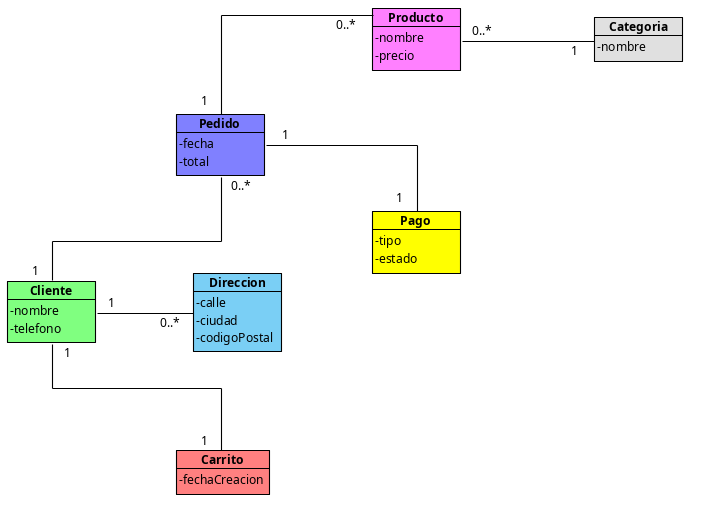
\includegraphics[width=0.85\textwidth]{figs/CasosdeUsoAnalisis.png}
    \caption{Diagrama de clases de análisis del sistema.}
    \label{fig:clases_analisis}
\end{figure}
\clearpage

\subsection{Diagrama de secuencia general del sistema (DSGS)}

La Figura~\ref{fig:dsgs} muestra el \textbf{diagrama de secuencia general del sistema (DSGS)}, 
que representa de forma dinámica las interacciones entre los principales actores externos 
y la \textit{WebApp}. En él se detalla el flujo completo de una compra, 
desde el inicio de sesión del cliente, la selección de productos y la realización del pedido, 
hasta la comunicación con la pasarela de pago \textit{Stripe}
y la notificación del resultado al \textit{bot de Telegram}. 
El diagrama también incluye un flujo alternativo en el que se muestra el manejo de un posible error de pago. 
Este modelo complementa al diagrama de casos de uso al ofrecer una visión temporal del comportamiento global del sistema.

\begin{figure}[H]
    \centering
    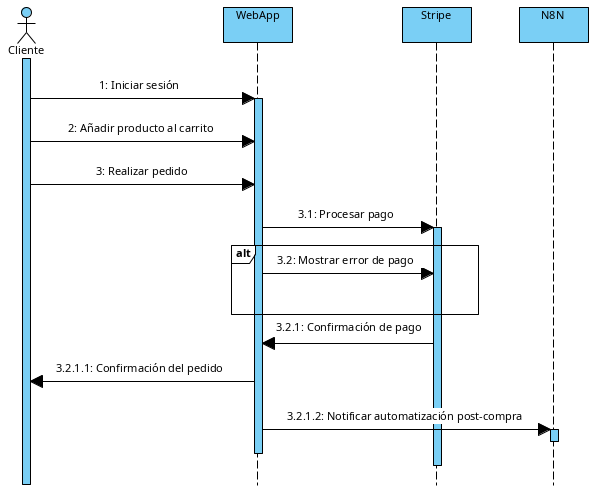
\includegraphics[width=0.9\textwidth]{figs/DSGS.png}
    \caption{Diagrama de secuencia general del sistema (DSGS).}
    \label{fig:dsgs}
\end{figure}
\subsubsection{DSGS-00 Diagrama de secuencia general del sistema}

\begin{table}[H]
\centering
\small
\begin{tabular}{|m{0.28\textwidth}|m{0.65\textwidth}|}
\hline
\textbf{Nombre} & DSGS-00 Diagrama de secuencia general del sistema \\ \hline

\textbf{Actor(es)} & Cliente, WebApp, Stripe, Bot de Telegram \\ \hline

\textbf{Descripción} &
Representa el flujo global del sistema durante el proceso de compra: inicio de sesión del cliente,
gestión del carrito, procesamiento del pago a través de Stripe y notificación del resultado al bot de Telegram,
incluyendo un flujo alternativo en caso de error de pago. \\ \hline

\textbf{Precondiciones} &
El cliente debe tener acceso a la WebApp y existir conexión con Stripe y el bot de Telegram. \\ \hline

\textbf{Postcondiciones} &
El pedido queda confirmado o rechazado, y el bot de Telegram recibe la notificación para ejecutar las tareas automáticas. \\ \hline

\textbf{Flujo principal} &
1. El cliente inicia sesión. \newline
2. Añade productos al carrito. \newline
3. Realiza el pedido. \newline
4. La WebApp envía el pago a Stripe. \newline
5. Stripe confirma el pago. \newline
6. La WebApp confirma el pedido. \newline
7. La WebApp notifica al bot de Telegram para ejecutar tareas post-compra. \\ \hline

\textbf{Flujos alternativos} &
4.a Stripe devuelve un error → la WebApp muestra el fallo al cliente. \\ \hline

\textbf{Requisitos funcionales relacionados} &
RF-01, RF-02, RF-04, RF-06 \\ \hline
\end{tabular}
\caption{Especificación del flujo DSGS-00 — Diagrama de secuencia del sistema.}
\end{table}

\clearpage



